\documentclass[notes xcolor=dvipsnames]{beamer}

\usetheme{Berkeley}

\setbeamertemplate{footline}[frame number]
%\setbeamertemplate{headline}{}

\usepackage{inputenc}
\usepackage{amsmath}
\usepackage{graphicx}
\usepackage{hyperref}

\title{Scheduling Weakly Consistent C Programs for Reconfigurable Hardware}
\subtitle{Nadesh Ramanathan, John Wickerson, George Constantinides.}

\author{Presented by \\ Akshay Gopalakrishnan}

\begin{document}
    
    \begin{frame}

        \maketitle

    \end{frame}

    \begin{frame}{Who are they?}

           \begin{columns}
                
            \begin{column}[]{0.3\textwidth}

                Yann Herklotz - PhD student supervised by John Wickerson, Imperial College London. 
                \begin{figure}
                    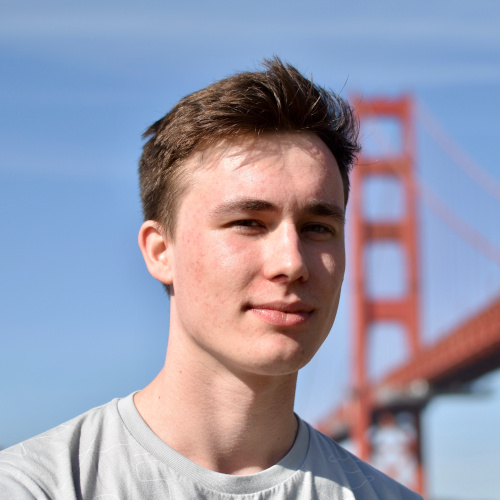
\includegraphics[scale=0.2]{YannHerklotz.jpg}
                \end{figure}
                
            \end{column}


            \begin{column}[]{0.3\textwidth}
                John Wickerson - Lecturer at Dept of Electrical and Electronic Engineering, Imperial College London.
                \begin{figure}
                    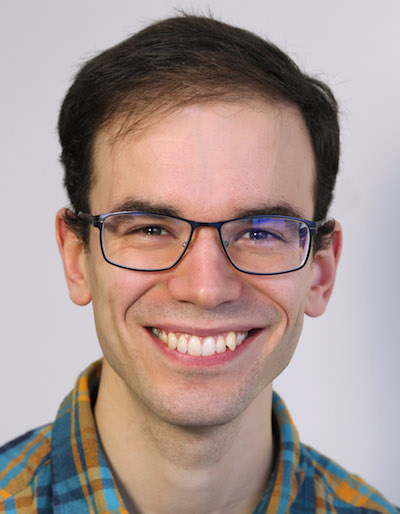
\includegraphics[scale=0.2]{john.jpg}
                \end{figure}
                
            \end{column}

            \begin{column}[]{0.3\textwidth}
                George Constantinides - Professor of Digital Computation, Imperial College London.
                \begin{figure}
                    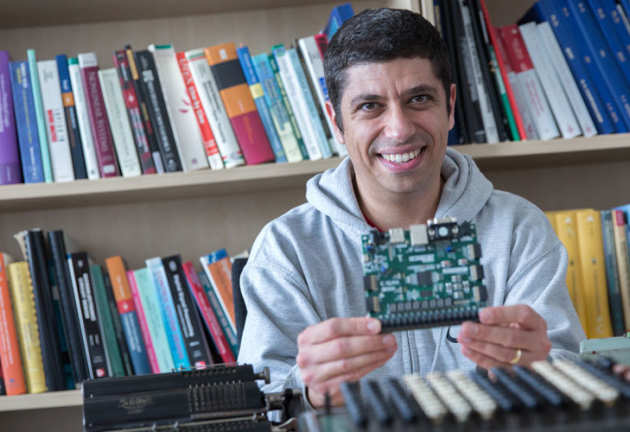
\includegraphics[scale=0.2]{Constantinides.jpg}
                \end{figure}
                
            \end{column}


        \end{columns}
    
    \end{frame}

    \section{Motivating Examples}
    
    %Example 1
    \subsection{Example 1}
    \begin{frame}{Scheduling Code block 1}

        %Put a set of questions here that this work is trying to answer
        \begin{columns}
            
            \begin{column}{0.5\textwidth}
                \begin{figure}
                    \makebox[\textwidth][c]{
                        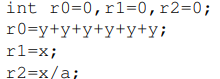
\includegraphics[scale=0.7]{RR-Part1.PNG}
                    }
                \end{figure}
                
            \end{column}

            \begin{column}{0.5\textwidth}

                \begin{figure}
                    \makebox[\textwidth][c]{
                        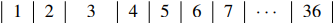
\includegraphics[scale=0.7]{RR-cycles.PNG}
                    }
                \end{figure}

                \begin{figure}
                    \makebox[\textwidth][c]{
                        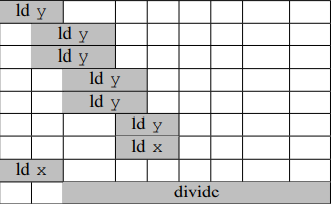
\includegraphics[scale=0.7]{RR-sched-part1.PNG}
                    }
                \end{figure}
                
            \end{column}


        \end{columns}
        
        

    \end{frame}

    \begin{frame}{Scheduling Code block 2}

        %Put a set of questions here that this work is trying to answer
        \begin{columns}
            
            \begin{column}{0.5\textwidth}
                \begin{figure}
                    \makebox[\textwidth][c]{
                        
\includegraphics[scale=0.7]{RR-part2.PNG}
                    }
                \end{figure}
                
            \end{column}

            \begin{column}{0.5\textwidth}

                \begin{figure}
                    \makebox[\textwidth][c]{
                        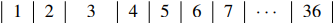
\includegraphics[scale=0.7]{RR-cycles.PNG}
                    }
                \end{figure}

                \begin{figure}
                    \makebox[\textwidth][c]{
                        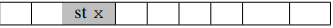
\includegraphics[scale=0.7]{RR-sched-part2.PNG}
                    }
                \end{figure}
                
            \end{column}


        \end{columns}
        
        

    \end{frame}

    \begin{frame}{Concurrent scheduling of Block 1 and 2}

        %Put a set of questions here that this work is trying to answer
        \begin{columns}
            
            \begin{column}{0.5\textwidth}
                \begin{figure}
                    \makebox[\textwidth][c]{
                        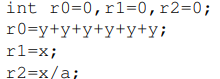
\includegraphics[scale=0.7]{RR-Part1.PNG}
                    }
                \end{figure}

                \begin{figure}
                    \makebox[\textwidth][c]{
                        \includegraphics[scale=0.7]{RR-Part2.PNG}
                    }
                \end{figure}

                \begin{figure}
                    \makebox[\textwidth][c]{
                        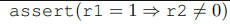
\includegraphics[scale=0.7]{RR-assert.PNG}
                    }
                \end{figure}

                
            \end{column}

            \begin{column}{0.5\textwidth}
                
                \begin{figure}
                    \makebox[\textwidth][c]{
                        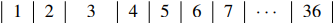
\includegraphics[scale=0.7]{RR-cycles.PNG}
                    }
                \end{figure}

                
                \begin{figure}
                    \makebox[\textwidth][c]{
                        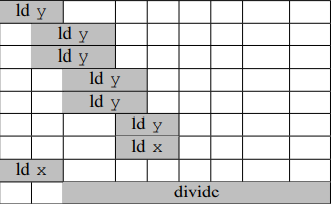
\includegraphics[scale=0.7]{RR-sched-part1.PNG}
                    }
                \end{figure}

                \begin{figure}
                    \makebox[\textwidth][c]{
                        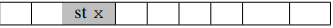
\includegraphics[scale=0.7]{RR-sched-part2.PNG}
                    }
                \end{figure}
                
            \end{column}


        \end{columns}
        
        

    \end{frame}

    \subsection{Example 2}
    \begin{frame}{Scheduling Code block 1}

        %Put a set of questions here that this work is trying to answer
        \begin{columns}
            
            \begin{column}{0.5\textwidth}
                \begin{figure}
                    \makebox[\textwidth][c]{
                        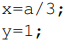
\includegraphics[scale=0.7]{WW-part1.PNG}
                    }
                \end{figure}
                
            \end{column}

            \begin{column}{0.5\textwidth}

                \begin{figure}
                    \makebox[\textwidth][c]{
                        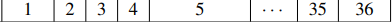
\includegraphics[scale=0.7]{WW-cycles.PNG}
                    }
                \end{figure}

                \begin{figure}
                    \makebox[\textwidth][c]{
                        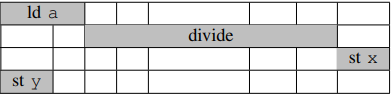
\includegraphics[scale=0.7]{WW-sched-part1.PNG}
                    }
                \end{figure}
                
            \end{column}


        \end{columns}
        
        

    \end{frame}

    \begin{frame}{Scheduling Code block 2}

        %Put a set of questions here that this work is trying to answer
        \begin{columns}
            
            \begin{column}{0.5\textwidth}
                \begin{figure}
                    \makebox[\textwidth][c]{
                        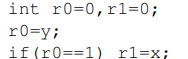
\includegraphics[scale=0.7]{WW-part2.PNG}
                    }
                \end{figure}
                
            \end{column}

            \begin{column}{0.5\textwidth}

                \begin{figure}
                    \makebox[\textwidth][c]{
                        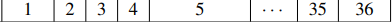
\includegraphics[scale=0.7]{WW-cycles.PNG}
                    }
                \end{figure}

                \begin{figure}
                    \makebox[\textwidth][c]{
                        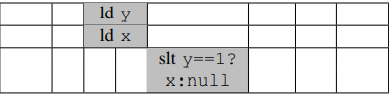
\includegraphics[scale=0.7]{WW-sched-part2.PNG}
                    }
                \end{figure}
                
            \end{column}


        \end{columns}
        
        

    \end{frame}


    \begin{frame}{Concurrent scheduling of Block 1 and 2}

        %Put a set of questions here that this work is trying to answer
        \begin{columns}
            
            \begin{column}{0.5\textwidth}
                \begin{figure}
                    \makebox[\textwidth][c]{
                        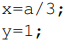
\includegraphics[scale=0.7]{WW-part1.PNG}
                    }
                \end{figure}

                \begin{figure}
                    \makebox[\textwidth][c]{
                        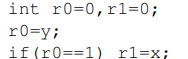
\includegraphics[scale=0.7]{WW-part2.PNG}
                    }
                \end{figure}

                \begin{figure}
                    \makebox[\textwidth][c]{
                        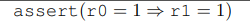
\includegraphics[scale=0.7]{WW-assert.PNG}
                    }
                \end{figure}
                
            \end{column}

            \begin{column}{0.5\textwidth}
                
                \begin{figure}
                    \makebox[\textwidth][c]{
                        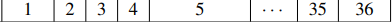
\includegraphics[scale=0.7]{WW-cycles.PNG}
                    }
                \end{figure}

                
                \begin{figure}
                    \makebox[\textwidth][c]{
                        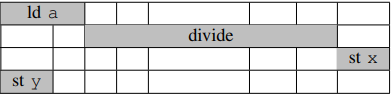
\includegraphics[scale=0.7]{WW-sched-part1.PNG}
                    }
                \end{figure}

                \begin{figure}
                    \makebox[\textwidth][c]{
                        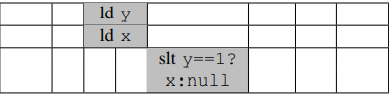
\includegraphics[scale=0.7]{WW-sched-part2.PNG}
                    }
                \end{figure}
                
            \end{column}


        \end{columns}
        
        

    \end{frame}

    \section{Problem}

    \subsection{Dependency}
    \begin{frame}{Data Dependencies: non-aliasing}


        \begin{figure}
            \makebox[\textwidth][c]{
                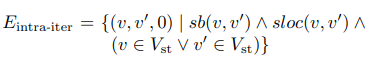
\includegraphics{IntraIter-Dep.PNG}
            }
        \end{figure}

        \begin{figure}
            \makebox[\textwidth][c]{
                \includegraphics{InterIter-Dep.PNG}
            }
        \end{figure}
        
    \end{frame}

    \subsection{SC Dependencies}
    \begin{frame}{Adding WW|WR|RW|RR Dependancies}

        \begin{figure}
            \makebox[\textwidth][c]{
                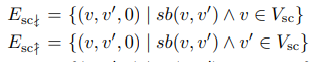
\includegraphics{SC-constraint.PNG}
            }
        \end{figure}

        \begin{columns}
            
            \begin{column}{0.5\textwidth}

                \begin{figure}
                    \makebox[\textwidth][c]{
                        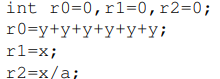
\includegraphics{RR-Part1.PNG}
                    }
                \end{figure}
                
            \end{column}

            \begin{column}{0.5\textwidth}
                
                \begin{figure}
                    \makebox[\textwidth][c]{
                        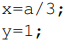
\includegraphics{WW-part1.PNG}
                    }
                \end{figure}

            \end{column}

        \end{columns}
        
    \end{frame}

    \begin{frame}{Final Dependency Expression}

        \begin{figure}
            \makebox[\textwidth][c]{
                \includegraphics{Strong-constraint.PNG}
            }
        \end{figure}
        
    \end{frame}
    
    \subsection{New Scheduling}
    \begin{frame}{Example}

        Without pipelining
        \begin{figure}
            \makebox[\textwidth][c]{
                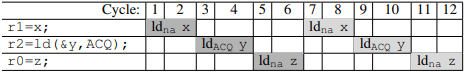
\includegraphics[scale=0.7]{Gen-ex-SC-no-pipe.PNG}
            }
        \end{figure}
             
        With pipelining
        \begin{figure}
            \makebox[\textwidth][c]{
                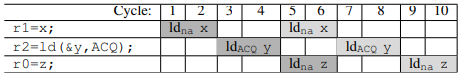
\includegraphics[scale=0.7]{Gen-ex-SC-pipe.PNG}
            }
        \end{figure}     
        
    \end{frame}

    \subsection{Rel-Acq Dependencies}
    \begin{frame}{Weakening: Adding Release-Acquire Dependencies}
        
        \begin{figure}
            \makebox[\textwidth][c]{
                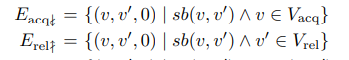
\includegraphics{Rel-Acq-Constraint.PNG}
            }
        \end{figure}

        
        \begin{columns}
            
            \begin{column}{0.5\textwidth}

                \begin{figure}
                    \makebox[\textwidth][c]{
                        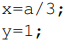
\includegraphics{WW-part1.PNG}
                    }
                \end{figure}
                
            \end{column}

            \begin{column}{0.5\textwidth}
                
                \begin{figure}
                    \makebox[\textwidth][c]{
                        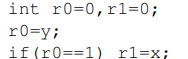
\includegraphics{WW-part2.PNG}
                    }
                \end{figure}

            \end{column}

        \end{columns}
    
    \end{frame}

    \begin{frame}{Adding RR Dependency}

            \begin{figure}
                \makebox[\textwidth][c]{
                    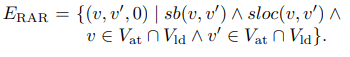
\includegraphics{RR-constraint.PNG}
                }
            \end{figure}
            
            \begin{figure}
                \makebox[\textwidth][c]{
                    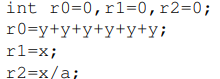
\includegraphics{RR-Part1.PNG}
                }
            \end{figure}
            
            
    \end{frame}

    \begin{frame}{Final Dependency Expression}

        \begin{figure}
            \makebox[\textwidth][c]{
                \includegraphics{Weak-constraint.PNG}
            }
        \end{figure}
        
    \end{frame}

    \subsection{New Scheduling}
    \begin{frame}{Example}

        Without pipelining
        \begin{figure}
            \makebox[\textwidth][c]{
                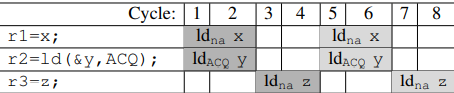
\includegraphics[scale=0.7]{Gen-ex-Acq-no-pipe.PNG}
            }
        \end{figure}
             
        With pipelining
        \begin{figure}
            \makebox[\textwidth][c]{
                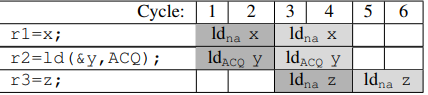
\includegraphics[scale=0.7]{Gen-ex-Acq-pipe.PNG}
            }
        \end{figure}     
        
    \end{frame}

    \section{Evaluation}

    \subsection{MP Example}
    \begin{frame}{Message Passing Algorithm}

        \begin{figure}
            \makebox[\textwidth][c]{
                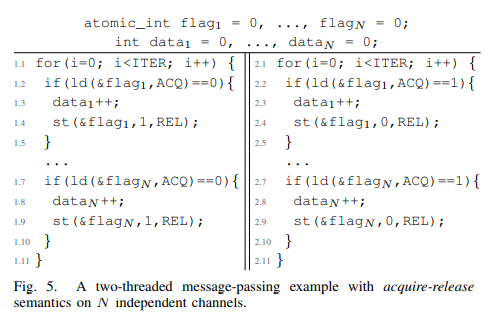
\includegraphics[scale=0.7]{MP-Acq-Rel.PNG}
            }
        \end{figure}
        
    \end{frame}


    \begin{frame}{Impact of Modified Scheduling}

        \begin{figure}
            \makebox[\textwidth][c]{
                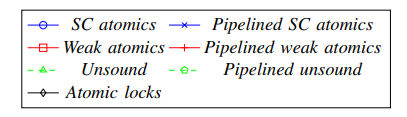
\includegraphics[scale=0.7]{MP-Legend.PNG}
            }
        \end{figure}

        \begin{figure}
            \makebox[\textwidth][c]{
                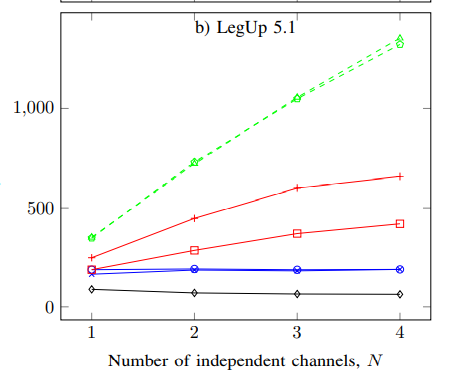
\includegraphics[scale=0.7]{MP_eval.PNG}
            }
        \end{figure}

        
    \end{frame}

    \begin{frame}{Resource Usage}
        \begin{figure}
            \makebox[\textwidth][c]{
                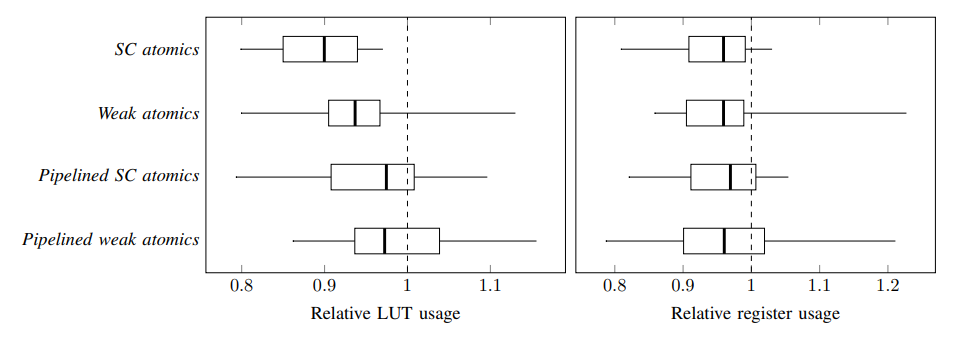
\includegraphics[scale=0.5]{LUT-Reg-Usage.PNG}
            }
        \end{figure}
        
    \end{frame}


    \subsection{Pros/Cons}

    \begin{frame}{Positives}

        \begin{itemize}
            \item New scheduling for programs with atomics.
            \item Do not require locks/notion of critical section for Hardware design.
            \item Efficient and correct scheduling  
        \end{itemize}

    \end{frame}

    \begin{frame}{Pending Work}

        \begin{itemize}
            \item Does not support Atomic Read-Modify-Write instructions. 
            \item Addressing other potential transformations (eg: Elimination, Introduction, Inlining, etc) for efficient scheduling. 
        \end{itemize}

    \end{frame}


    \begin{frame}{Thank you}

        \begin{itemize}
            \item \href{https://johnwickerson.wordpress.com/2017/02/23/translating-lock-free-relaxed-concurrency-from-software-into-hardware/}{John's Blog}
            \item \href{https://dl.acm.org/doi/10.1145/3020078.3021733}{Previous Work}
            \item \href{https://github.com/nadeshr/weak_atomics}{Testing+Verification}
        \end{itemize}

        Questions?

    \end{frame}


\end{document}